\documentclass[journal,12pt,twocolumn]{IEEEtran}
%
\usepackage{setspace}
\usepackage{gensymb}
%\doublespacing
\singlespacing

%\usepackage{graphicx}
%\usepackage{amssymb}
%\usepackage{relsize}
\usepackage[cmex10]{amsmath}
\usepackage{siunitx}
%\usepackage{amsthm}
%\interdisplaylinepenalty=2500
%\savesymbol{iint}
%\usepackage{txfonts}
%\restoresymbol{TXF}{iint}
%\usepackage{wasysym}
\usepackage{amsthm}
\usepackage{iithtlc}
\usepackage{mathrsfs}
\usepackage{txfonts}
\usepackage{stfloats}
\usepackage{steinmetz}
\usepackage{supertabular}
%\usepackage{bm}
\usepackage{cite}
\usepackage{cases}
\usepackage{subfig}
%\usepackage{xtab}
\usepackage{longtable}
\usepackage{multirow}
%\usepackage{algorithm}
%\usepackage{algpseudocode}
\usepackage{enumitem}
\usepackage{mathtools}
\usepackage{tikz}
\usepackage{circuitikz}
\usepackage{verbatim}
\usepackage{tfrupee}
\usepackage[breaklinks=true]{hyperref}
%\usepackage{stmaryrd}
\usepackage{tkz-euclide} % loads  TikZ and tkz-base
%\usetkzobj{all}
\usetikzlibrary{calc,math}
\usetikzlibrary{fadings}
\usepackage{listings}
    \usepackage{color}                                            %%
    \usepackage{array}                                            %%
    \usepackage{longtable}                                        %%
    \usepackage{calc}                                             %%
    \usepackage{multirow}                                         %%
    \usepackage{hhline}                                           %%
    \usepackage{ifthen}                                           %%
  %optionally (for landscape tables embedded in another document): %%
    \usepackage{lscape}     
\usepackage{multicol}
\usepackage{chngcntr}
\usepackage{blkarray}
\usepackage{karnaugh-map}
\usepackage{fontspec}
\usepackage[intoc]{nomencl}
\makenomenclature

%\usetikzlibrary{arrows, shapes.gates.logic.US, calc}
\usetikzlibrary{arrows,shapes.gates.logic.US,shapes.gates.logic.IEC,calc}
%\setmainfont{Sanskrit_2003.ttf}
\setmainfont{Nakula.ttf}
%\setmainfont{Lohit-Devanagari.ttf}


%\usepackage{enumerate}

%\usepackage{wasysym}
%\newcounter{MYtempeqncnt}
\DeclareMathOperator*{\Res}{Res}
%\renewcommand{\baselinestretch}{2}
\renewcommand\thesection{\arabic{section}}
\renewcommand\thesubsection{\thesection.\arabic{subsection}}
\renewcommand\thesubsubsection{\thesubsection.\arabic{subsubsection}}

\renewcommand\thesectiondis{\arabic{section}}
\renewcommand\thesubsectiondis{\thesectiondis.\arabic{subsection}}
\renewcommand\thesubsubsectiondis{\thesubsectiondis.\arabic{subsubsection}}

% correct bad hyphenation here
\hyphenation{op-tical net-works semi-conduc-tor}
\def\inputGnumericTable{}                                 %%

\lstset{
%language=C,
frame=single, 
breaklines=true,
columns=fullflexible
}
%\lstset{
%language=tex,
%frame=single, 
%breaklines=true
%}

\begin{document}
%


\newtheorem{theorem}{Theorem}[section]
\newtheorem{problem}{Problem}
\newtheorem{proposition}{Proposition}[section]
\newtheorem{lemma}{Lemma}[section]
\newtheorem{corollary}[theorem]{Corollary}
\newtheorem{example}{Example}[section]
\newtheorem{definition}[problem]{Definition}
%\newtheorem{thm}{Theorem}[section] 
%\newtheorem{defn}[thm]{Definition}
%\newtheorem{algorithm}{Algorithm}[section]
%\newtheorem{cor}{Corollary}
\newcommand{\BEQA}{\begin{eqnarray}}
\newcommand{\EEQA}{\end{eqnarray}}
\newcommand{\define}{\stackrel{\triangle}{=}}

\bibliographystyle{IEEEtran}
%\bibliographystyle{ieeetr}


\providecommand{\mbf}{\mathbf}
\providecommand{\pr}[1]{\ensuremath{\Pr\left(#1\right)}}
\providecommand{\qfunc}[1]{\ensuremath{Q\left(#1\right)}}
\providecommand{\sbrak}[1]{\ensuremath{{}\left[#1\right]}}
\providecommand{\lsbrak}[1]{\ensuremath{{}\left[#1\right.}}
\providecommand{\rsbrak}[1]{\ensuremath{{}\left.#1\right]}}
\providecommand{\brak}[1]{\ensuremath{\left(#1\right)}}
\providecommand{\lbrak}[1]{\ensuremath{\left(#1\right.}}
\providecommand{\rbrak}[1]{\ensuremath{\left.#1\right)}}
\providecommand{\cbrak}[1]{\ensuremath{\left\{#1\right\}}}
\providecommand{\lcbrak}[1]{\ensuremath{\left\{#1\right.}}
\providecommand{\rcbrak}[1]{\ensuremath{\left.#1\right\}}}
\providecommand{\ceil}[1]{\left \lceil #1 \right \rceil }
\theoremstyle{remark}
\newtheorem{rem}{Remark}
\newcommand{\sgn}{\mathop{\mathrm{sgn}}}
\providecommand{\abs}[1]{\left\vert#1\right\vert}
\providecommand{\res}[1]{\Res\displaylimits_{#1}} 
\providecommand{\norm}[1]{\left\lVert#1\right\rVert}
%\providecommand{\norm}[1]{\lVert#1\rVert}
\providecommand{\mtx}[1]{\mathbf{#1}}
\providecommand{\mean}[1]{E\left[ #1 \right]}
\providecommand{\fourier}{\overset{\mathcal{F}}{ \rightleftharpoons}}
%\providecommand{\hilbert}{\overset{\mathcal{H}}{ \rightleftharpoons}}
\providecommand{\system}{\overset{\mathcal{H}}{ \longleftrightarrow}}
	%\newcommand{\solution}[2]{\textbf{Solution:}{#1}}
\newcommand{\solution}{\noindent \textbf{Solution: }}
\newcommand{\cosec}{\,\text{cosec}\,}
\providecommand{\dec}[2]{\ensuremath{\overset{#1}{\underset{#2}{\gtrless}}}}
\newcommand{\myvec}[1]{\ensuremath{\begin{pmatrix}#1\end{pmatrix}}}
\newcommand{\mydet}[1]{\ensuremath{\begin{vmatrix}#1\end{vmatrix}}}
%\numberwithin{equation}{section}
\numberwithin{equation}{subsection}
%\numberwithin{problem}{section}
%\numberwithin{definition}{section}
\makeatletter
\@addtoreset{figure}{problem}
\makeatother

\let\StandardTheFigure\thefigure
\let\vec\mathbf
%\renewcommand{\thefigure}{\theproblem.\arabic{figure}}
%\renewcommand{\thefigure}{\theproblem}
\renewcommand{\thefigure}{\thesection}
%\setlist[enumerate,1]{before=\renewcommand\theequation{\theenumi.\arabic{equation}}
%\counterwithin{equation}{enumi}


%\renewcommand{\theequation}{\arabic{subsection}.\arabic{equation}}

\def\putbox#1#2#3{\makebox[0in][l]{\makebox[#1][l]{}\raisebox{\baselineskip}[0in][0in]{\raisebox{#2}[0in][0in]{#3}}}}
     \def\rightbox#1{\makebox[0in][r]{#1}}
     \def\centbox#1{\makebox[0in]{#1}}
     \def\topbox#1{\raisebox{-\baselineskip}[0in][0in]{#1}}
     \def\midbox#1{\raisebox{-0.5\baselineskip}[0in][0in]{#1}}

\vspace{3cm}

\title{
%	\logo{
अंकीय तर्क विधि
%	}
}
\author{ गाड़ेपल्लि वेंकट विश्वनाथ शर्मा $^{*}$% <-this % stops a space
	\thanks{*रचयिता भारतीय प्रौद्योगिकी संस्थान, हैदराबाद,५०२२८५ के विद्युत अभियान्त्रिकी विभाग में कार्यरत हैं, ईमेल:gadepall@ee.iith.ac.in। यह आलेख मुक्त स्रोत विचारधारा के अनुरूप  है।}
	
}	
%\title{
%	\logo{Matrix Analysis through Octave}{\begin{center}\includegraphics[scale=.24]{tlc}\end{center}}{}{HAMDSP}
%}


% paper title
% can use linebreaks \\ within to get better formatting as desired
%\title{Matrix Analysis through Octave}
%
%
% author names and IEEE memberships
% note positions of commas and nonbreaking spaces ( ~ ) LaTeX will not break
% a structure at a ~ so this keeps an author's name from being broken across
% two lines.
% use \thanks{} to gain access to the first footnote area
% a separate \thanks must be used for each paragraph as LaTeX2e's \thanks
% was not built to handle multiple paragraphs
%

%\author{<-this % stops a space
%\thanks{}}
%}
% note the % following the last \IEEEmembership and also \thanks - 
% these prevent an unwanted space from occurring between the last author name
% and the end of the author line. i.e., if you had this:
% 
% \author{....lastname \thanks{...} \thanks{...} }
%                     ^------------^------------^----Do not want these spaces!
%
% a space would be appended to the last name and could cause every name on that
% line to be shifted left slightly. This is one of those "LaTeX things". For
% instance, "\textbf{A} \textbf{B}" will typeset as "A B" not "AB". To get
% "AB" then you have to do: "\textbf{A}\textbf{B}"
% \thanks is no different in this regard, so shield the last } of each \thanks
% that ends a line with a % and do not let a space in before the next \thanks.
% Spaces after \IEEEmembership other than the last one are OK (and needed) as
% you are supposed to have spaces between the names. For what it is worth,
% this is a minor point as most people would not even notice if the said evil
% space somehow managed to creep in.



% The paper headers
%\markboth{Journal of \LaTeX\ Class Files,~Vol.~6, No.~1, January~2007}%
%{Shell \MakeLowercase{\textit{et al.}}: Bare Demo of IEEEtran.cls for Journals}
% The only time the second header will appear is for the odd numbered pages
% after the title page when using the twoside option.
% 
% *** Note that you probably will NOT want to include the author's ***
% *** name in the headers of peer review papers.                   ***
% You can use \ifCLASSOPTIONpeerreview for conditional compilation here if
% you desire.




% If you want to put a publisher's ID mark on the page you can do it like
% this:
%\IEEEpubid{0000--0000/00\$00.00~\copyright~2007 IEEE}
% Remember, if you use this you must call \IEEEpubidadjcol in the second
% column for its text to clear the IEEEpubid mark.



% make the title area
\maketitle

\newpage

\tableofcontents


\bigskip

\renewcommand{\thefigure}{\theenumi}
\renewcommand{\thetable}{\theenumi}
\renewcommand{\abstractname}{सार}
\renewcommand{\nomname}{नामकरण}
\renewcommand{\solution}{हल: }
\renewcommand{\figurename}{आकृति.}
\renewcommand{\tablename}{सारणी.}
%\renewcommand{\theequation}{\theenumi}

%\begin{abstract}
%%\boldmath
%In this letter, an algorithm for evaluating the exact analytical bit error rate  (BER)  for the piecewise linear (PL) combiner for  multiple relays is presented. Previous results were available only for upto three relays. The algorithm is unique in the sense that  the actual mathematical expressions, that are prohibitively large, need not be explicitly obtained. The diversity gain due to multiple relays is shown through plots of the analytical BER, well supported by simulations. 
%
%\end{abstract}
% IEEEtran.cls defaults to using nonbold math in the Abstract.
% This preserves the distinction between vectors and scalars. However,
% if the journal you are submitting to favors bold math in the abstract,
% then you can use LaTeX's standard command \boldmath at the very start
% of the abstract to achieve this. Many IEEE journals frown on math
% in the abstract anyway.

% Note that keywords are not normally used for peerreview papers.
%\begin{IEEEkeywords}
%Cooperative diversity, decode and forward, piecewise linear
%\end{IEEEkeywords}



% For peer review papers, you can put extra information on the cover
% page as needed:
% \ifCLASSOPTIONpeerreview
% \begin{center} \bfseries EDICS Category: 3-BBND \end{center}
% \fi
%
% For peerreview papers, this IEEEtran command inserts a page break and
% creates the second title. It will be ignored for other modes.
%\IEEEpeerreviewmaketitle

\begin{abstract}
यह लेख प्राथमिक विद्यालयों से लेकर  विश्व विद्यालयों तक सभी  छात्रों को एक सरल विधि से अंकीय तर्क  से अवगत करने का प्रयास है।  
%ॐ श्री गणेशाय नमः॥
%\\
%\indent जय श्री राम।
%This manual provides a simple introduction to Digital Design.
\end{abstract}

%\section{Nomenclature}
\printnomenclature[1.7in]
\input{hindi/nomen.tex}


\section{सप्तांश   प्रदर्शी }
%\subsection{Introduction}
\renewcommand{\theequation}{\theenumi}
\renewcommand{\thefigure}{\theenumi}
\begin{enumerate}[label=\thesection.\arabic*.,ref=\thesection.\theenumi]
\numberwithin{equation}{enumi}
\numberwithin{figure}{enumi}
\numberwithin{table}{enumi}

\item  Fig. \ref{fig:sevenseg} shows a seven segment display with pins $a,b,c,d,e,f,g$.  Each of these pins is connected to an LED (light emitting device).

\begin{figure}[!ht]
\centering
\resizebox {\columnwidth} {!} {
%\subsection{Introduction}
\renewcommand{\theequation}{\theenumi}
\renewcommand{\thefigure}{\theenumi}
\begin{enumerate}[label=\thesection.\arabic*.,ref=\thesection.\theenumi]
\numberwithin{equation}{enumi}
\numberwithin{figure}{enumi}
\numberwithin{table}{enumi}

\item  Fig. \ref{fig:sevenseg} shows a seven segment display with pins $a,b,c,d,e,f,g$.  Each of these pins is connected to an LED (light emitting device).

\begin{figure}[!ht]
\centering
\resizebox {\columnwidth} {!} {
%\subsection{Introduction}
\renewcommand{\theequation}{\theenumi}
\renewcommand{\thefigure}{\theenumi}
\begin{enumerate}[label=\thesection.\arabic*.,ref=\thesection.\theenumi]
\numberwithin{equation}{enumi}
\numberwithin{figure}{enumi}
\numberwithin{table}{enumi}

\item  Fig. \ref{fig:sevenseg} shows a seven segment display with pins $a,b,c,d,e,f,g$.  Each of these pins is connected to an LED (light emitting device).

\begin{figure}[!ht]
\centering
\resizebox {\columnwidth} {!} {
\input{./figs/sevenseg.tex}
}
\caption{}
\label{fig:sevenseg}
\end{figure}

\item Fig. \ref{fig:sevenseg12} shows how to generate the numbers on the display using Table
\ref{table:arduioport}.  Complete Table \ref{table:arduioport} by drawing the figures for all numbers from 0-9.

\begin{figure}[!h]
\begin{center}
\resizebox {\columnwidth} {!} {
\input{./figs/sevenseg12.tex}
}
\end{center}
\caption{}
\label{fig:sevenseg12}
\end{figure}


\begin{table}[!h]
\centering
\input{./tables/arduinoport.tex}
\caption{}
\label{table:arduioport}
\end{table}


\end{enumerate}

}
\caption{}
\label{fig:sevenseg}
\end{figure}

\item Fig. \ref{fig:sevenseg12} shows how to generate the numbers on the display using Table
\ref{table:arduioport}.  Complete Table \ref{table:arduioport} by drawing the figures for all numbers from 0-9.

\begin{figure}[!h]
\begin{center}
\resizebox {\columnwidth} {!} {
\input{./figs/sevenseg12.tex}
}
\end{center}
\caption{}
\label{fig:sevenseg12}
\end{figure}


\begin{table}[!h]
\centering
\input{./tables/arduinoport.tex}
\caption{}
\label{table:arduioport}
\end{table}


\end{enumerate}

}
\caption{}
\label{fig:sevenseg}
\end{figure}

\item Fig. \ref{fig:sevenseg12} shows how to generate the numbers on the display using Table
\ref{table:arduioport}.  Complete Table \ref{table:arduioport} by drawing the figures for all numbers from 0-9.

\begin{figure}[!h]
\begin{center}
\resizebox {\columnwidth} {!} {
\input{./figs/sevenseg12.tex}
}
\end{center}
\caption{}
\label{fig:sevenseg12}
\end{figure}


\begin{table}[!h]
\centering
\input{./tables/arduinoport.tex}
\caption{}
\label{table:arduioport}
\end{table}


\end{enumerate}

\section{परवर्ती गूढ़वाचक}
\renewcommand{\theequation}{\theenumi}
\renewcommand{\thefigure}{\theenumi}
\begin{enumerate}[label=\thesection.\arabic*.,ref=\thesection.\theenumi]
\numberwithin{equation}{enumi}
\numberwithin{figure}{enumi}
\numberwithin{table}{enumi}

\item The incrementing decoder   takes the numbers $0,1,\dots,9$ in binary as inputs and generates
the consecutive number as output.  The corresponding {\em truth table} is available in Table. \ref{table:counter_decoder}.
%\onecolumn
\begin{table}[!h]
\centering
%\resizebox{\columnwidth}{!}
%{
\input{./tables/counter_decoder}
%}
\caption{Truth table for the incrementing decoder}
\label{table:counter_decoder}
\end{table}
\item Using Boolean logic, outputs $A, B, C$ and $D$  in Table \ref{table:counter_decoder} can be expressed in terms of the inputs $W,X,Y,Z$ as
%
\begin{align}
\label{eq:inc_A}
A &= W^{\prime}X^{\prime}Y^{\prime}Z^{\prime} + W^{\prime}XY^{\prime}Z^{\prime}
+W^{\prime}X^{\prime}YZ^{\prime}
\nonumber \\
 & \quad +W^{\prime}XYZ^{\prime}
+W^{\prime}X^{\prime}Y^{\prime}Z
\\
\label{eq:inc_B}
B &= WX^{\prime}Y^{\prime}Z^{\prime} + W^{\prime}XY^{\prime}Z^{\prime}
\nonumber \\ 
& \quad 
+WX^{\prime}YZ^{\prime}
+W^{\prime}XYZ^{\prime}
\\
\label{eq:inc_C}
C &= WXY^{\prime}Z^{\prime} + W^{\prime}X^{\prime}YZ^{\prime}
\nonumber \\ 
& \quad 
+WX^{\prime}YZ^{\prime}
+W^{\prime}XYZ^{\prime}
\\
D &= WXYZ^{\prime} + W^{\prime}X^{\prime}Y^{\prime}Z
\label{eq:inc_D}
\end{align}
\item Execute the following code for different input values to verify \eqref{eq:inc_A}-\eqref{eq:inc_D}.
\label{code:inc_decode}
\begin{lstlisting}
codes/inc_decode.c
\end{lstlisting}
%\item Modify the above C code to verify \eqref{eq:inc_A}, \eqref{eq:inc_B}
%and \eqref{eq:inc_C}.
%
%\item Repeat the exercise for the truth table in \ref{table:disp_dec}.
%%
%\begin{table}
%\centering
%\input{./tables/disp_dec.tex}
%\caption{Truth table for display decoder.}
%\label{table:disp_dec}
%\end{table}

\end{enumerate}
%
%

\section{प्रदर्शी गूढ़वाचक}
\input{hindi/dispdec.tex}
%
\section{कार्नो मानचित्र}
\subsection{परवर्ती गूढ़वाचक}
\input{hindi/kmap_inc.tex}
\subsection{प्रदर्शी गूढ़वाचक}
\input{hindi/kmap_disp.tex}
%
\section{निर्गुण अवस्था}
\subsection{परवर्ती गूढ़वाचक}
\renewcommand{\theequation}{\theenumi}
\renewcommand{\thefigure}{\theenumi}
\begin{enumerate}[label=\thesubsection.\arabic*.,ref=\thesubsection.\theenumi]
\numberwithin{equation}{enumi}
\numberwithin{figure}{enumi}
\numberwithin{table}{enumi}


\item Obtain the expression for $B$ using Fig. \ref{fig:inc_kmapX_B}


\solution

\begin{align}
\label{eq:kmapX_inc_B}
B=W^{\prime}X+WX^{\prime}Z^{\prime}
\end{align}
%
where $\oplus$ denotes the XOR operation.
\begin{figure}[!ht]
\centering
\resizebox{\columnwidth}{!} {
\tikzstyle{branch}=[fill,shape=circle,minimum size=3pt,inner sep=0pt]
\begin{tikzpicture}[label distance=2mm]

    \node (x1) at (0,0) {$W$};
    \node (x2) at (0,-2.5) {$X$};
    \node (x3) at (0,-6) {$Z$};
    
    \node[and gate US, draw, logic gate inputs=nnnnnnnnn] at ($(x1)+(5,-2)$) (And1) {};
    \node[and gate US, draw, logic gate inputs=nnnnnnnnn] at ($(x3)+(5,-1)$) (And2) {};
    
    \node[or gate US, draw, logic gate inputs=nnnnnnnnnnnn, anchor=input 1] at ($(And2.output)+(3,3.5)$) (Or1) {};
    
 \draw (x1)--(2,0)
  (2,0)--(2,-2)
  (2,-2)--(4,-2);
  \draw (x2)--(4,-2.5);
  \draw (3.9,-2) node[american] {O};
  \draw (6.1,-2)--(7.2,-2)
  (7.2,-2)--(7.2,-3.9)
  (7.2,-3.9)--(9.3,-3.9);
  \draw (12,-4.5)--(14,-4.5);
  \draw (x3)--(1,-6)
  (1,-6)--(1,-7.6)
  (1,-7.6)--(4,-7.6);
  \draw (3.9,-7.6) node[american] {O};
  \draw (1,-2.5)--(1,-5)
  (1,-5)--(3.4,-5)
  (3.4,-5)--(3.4,-6.4)
  (3.4,-6.4)--(4,-6.4);
  \draw (3.9,-6.4) node[american] {O};
  \draw (6.1,-7)--(7.2,-7)
   (7.2,-7)--(7.2,-5)
  (7.2,-5)--(9.3,-5);
  \draw (1,0)--(1,-1)
  (1,-1)--(-1,-1)
  (-1,-1)--(-1,-5.5)
  (-1,-5.5)--(2,-5.5)
  (2,-5.5)--(2,-6.9)
  (2,-6.9)--(4,-6.9);  
  
\end{tikzpicture}


}
\caption{K-map for $B$.}
\label{fig:inc_kmapX_B}
\end{figure}
%
\item Obtain the expression for $C$ using Fig. \ref{fig:inc_kmapX_C}
\begin{align}
\label{eq:kmapX_inc_C}
C = Y^{\prime}X+W^{\prime}XZ^{\prime}+YX^{\prime}
\end{align}
%
\begin{figure}[!ht]
\centering
\resizebox{\columnwidth}{!} {
\begin{karnaugh-map}[4][4][1][][]
    \minterms{3,4,5,6}
    \maxterms{0,1,2,7,8,9,10,11,12,13,14,15}
    \implicant{12}{10}
    \implicant{0}{1}
    \implicant{15}{7}
    \implicantcorner
    
    % note: position for start of \draw is (0, Y) where Y is
    % the Y size(number of cells high) in this case Y=2
    \draw[color=black, ultra thin] (0, 4) --
    node [pos=0.7, above right, anchor=south west] {$XW$} % YOU CAN CHANGE NAME OF VAR HERE, THE $X$ IS USED FOR ITALICS
    node [pos=0.7, below left, anchor=north east] {$ZY$} % SAME FOR THIS
    ++(135:1);
        
    \end{karnaugh-map}

}
\caption{K-map for $C$.}
\label{fig:inc_kmapX_C}
\end{figure}
\end{enumerate}

\subsection{प्रदर्शी गूढ़वाचक}
\renewcommand{\theequation}{\theenumi}
\renewcommand{\thefigure}{\theenumi}
\begin{enumerate}[label=\thesubsection.\arabic*.,ref=\thesubsection.\theenumi]
\numberwithin{equation}{enumi}
\numberwithin{figure}{enumi}
\numberwithin{table}{enumi}

\item Obtain the expression for $b$ using Fig. \ref{fig:disp_kmapX_b}
%
\solution
\begin{align}
\label{eq:kmap_dispX_b}
b=B^{\prime}+CD+C^{\prime}D^{\prime}
\end{align}
%
\begin{figure}[!ht]
\centering
\resizebox{\columnwidth}{!} {
\input{figs/disp/kmapX/b.tex}
}
\caption{K-map for $b$ using don't care.}
\label{fig:disp_kmapX_b}
\end{figure}

%
\end{enumerate}
%

%
\section{तर्क द्वार}
\renewcommand{\theequation}{\theenumi}
\renewcommand{\thefigure}{\theenumi}
\begin{enumerate}[label=\thesection.\arabic*.,ref=\thesection.\theenumi]
\numberwithin{equation}{enumi}
\numberwithin{figure}{enumi}
\numberwithin{table}{enumi}

\item The following equation is implemented using gates in Fig. \ref{fig:gates_B}
\begin{align}
B=W^{\prime}X+WX^{\prime}Z^{\prime}
\end{align}
\begin{figure}[!ht]
\begin{center}
\resizebox {\columnwidth} {!} {
\tikzstyle{branch}=[fill,shape=circle,minimum size=3pt,inner sep=0pt]
\begin{tikzpicture}[label distance=2mm]

    \node (x1) at (0,0) {$W$};
    \node (x2) at (0,-2.5) {$X$};
    \node (x3) at (0,-6) {$Z$};
    
    \node[and gate US, draw, logic gate inputs=nnnnnnnnn] at ($(x1)+(5,-2)$) (And1) {};
    \node[and gate US, draw, logic gate inputs=nnnnnnnnn] at ($(x3)+(5,-1)$) (And2) {};
    
    \node[or gate US, draw, logic gate inputs=nnnnnnnnnnnn, anchor=input 1] at ($(And2.output)+(3,3.5)$) (Or1) {};
    
 \draw (x1)--(2,0)
  (2,0)--(2,-2)
  (2,-2)--(4,-2);
  \draw (x2)--(4,-2.5);
  \draw (3.9,-2) node[american] {O};
  \draw (6.1,-2)--(7.2,-2)
  (7.2,-2)--(7.2,-3.9)
  (7.2,-3.9)--(9.3,-3.9);
  \draw (12,-4.5)--(14,-4.5);
  \draw (x3)--(1,-6)
  (1,-6)--(1,-7.6)
  (1,-7.6)--(4,-7.6);
  \draw (3.9,-7.6) node[american] {O};
  \draw (1,-2.5)--(1,-5)
  (1,-5)--(3.4,-5)
  (3.4,-5)--(3.4,-6.4)
  (3.4,-6.4)--(4,-6.4);
  \draw (3.9,-6.4) node[american] {O};
  \draw (6.1,-7)--(7.2,-7)
   (7.2,-7)--(7.2,-5)
  (7.2,-5)--(9.3,-5);
  \draw (1,0)--(1,-1)
  (1,-1)--(-1,-1)
  (-1,-1)--(-1,-5.5)
  (-1,-5.5)--(2,-5.5)
  (2,-5.5)--(2,-6.9)
  (2,-6.9)--(4,-6.9);  
  
\end{tikzpicture}


}
\end{center}
\caption{}
\label{fig:gates_B}
\end{figure}
\item The following equation is implemented using gates in Fig. \ref{fig:gates_b}
\begin{align}
b=B^{\prime}+CD+C^{\prime}D^{\prime}
\end{align}
\begin{figure}[!ht]
\begin{center}
\resizebox {\columnwidth} {!} {
\input{./figs/gates/b_disp.tex}
}
\end{center}
\caption{}
\label{fig:gates_b}
\end{figure}
\item The following equation is implemented using gates in Fig. \ref{fig:gates_a}
\begin{align}
    a=B^{\prime}D^{\prime}(A^{\prime}C+AC^{\prime})
\end{align}
\begin{figure}[!ht]
\begin{center}
\resizebox {\columnwidth} {!} {




\begin{circuitikz}
 \draw
(0,-1)node[xor port](myxor1){}

(2,2)node[and port](myand2){}

(4,1)node[and port](myand3){}

(-0.5,0.7)node[not port](mynot4){}

(-0.5,2.3)node[not port](mynot5) {}

(myxor1.out)--(myand3.in 2)
(myand2.out)--(myand3.in 1)
(mynot4.out)--(myand2.in 2)
(mynot5.out)--(myand2.in 1);

\node(x3) at (-1.6,-1.3) {$C$};
\node(x2) at (-1.6,-0.7) {$A$}; 
\node(x1) at (-1.6,0.7) {$D$};
\node(x0) at (-1.6,2.3) {$B$};
\node(x3) at (6,1) {$B'D'(A'C+AC')$};

\end{circuitikz}



}
\end{center}
\caption{}
\label{fig:gates_a}
\end{figure}
%
\item The following equation is implemented using gates in Fig. \ref{fig:gates_d}
\begin{align}
d = AB^{\prime}C^{\prime}+A^{\prime}B^{\prime}CD^{\prime}+ABCD^{\prime}
\end{align}
\begin{figure}[!ht]
\begin{center}
\resizebox {\columnwidth} {!} {
\tikzstyle{branch}=[fill,shape=circle,minimum size=3pt,inner sep=0pt]
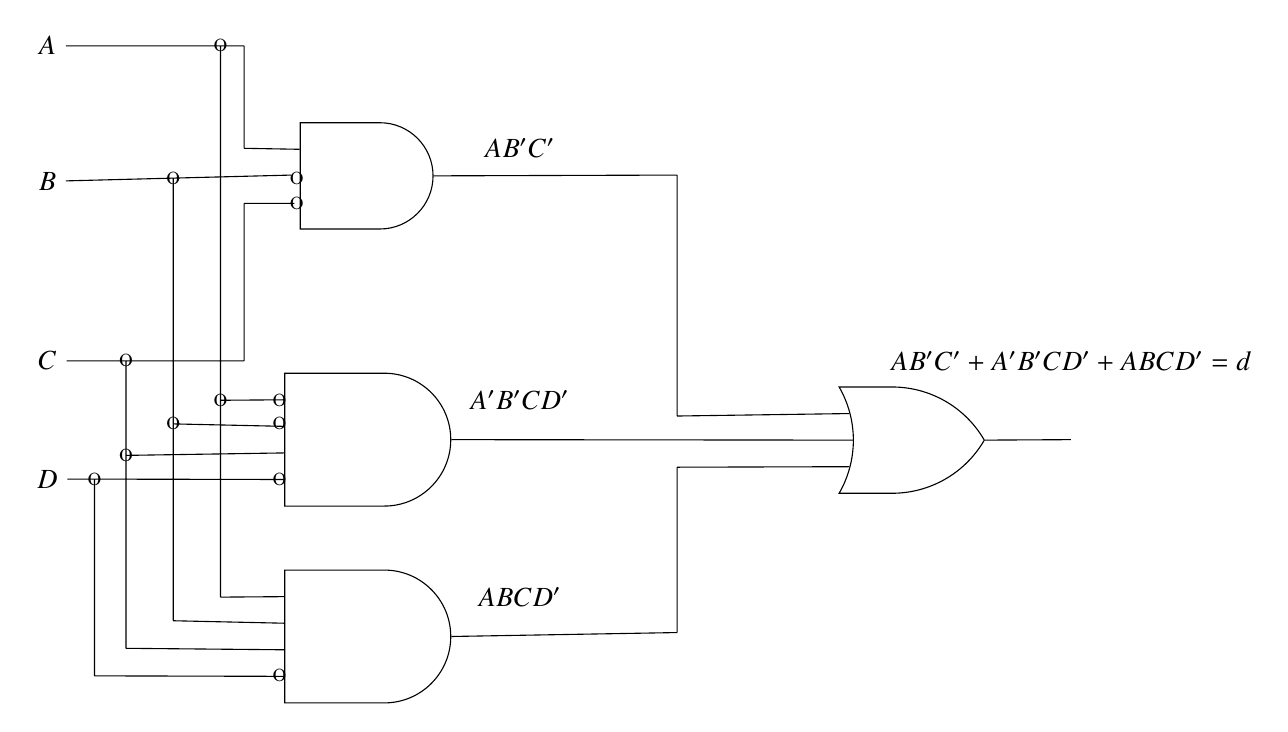
\begin{tikzpicture}[label distance=2mm]
    \node (x1) at (0,0) {$A$};
    \node (x2) at (0,-1.72) {$B$};
    \node (x3) at (0,-4) {$C$};
    \node (x4) at (0,-5.5) {$D$};
    
    \node[and gate US, draw, logic gate inputs=nnnnnnn] at ($(x1)+(4,-1.65)$) (And1) {};
    \node[and gate US, draw, logic gate inputs=nnnnnnnnn] at ($(x3)+(4,-1)$) (And2) {};
    \node[and gate US, draw, logic gate inputs=nnnnnnnnn] at ($(x4)+(4,-2)$) (And3) {};
    
    \node[or gate US, draw, logic gate inputs=nnnnnnn, anchor=input 1] at ($(And2.output)+(5,0.5)$) (Or1) {};
    
 \draw (x1)--(2.5,0) 
   (2.5,0)--(2.5,-1.3) 
   (2.5,-1.3)--(And1.input 2)
   (x2)--(3.1,-1.64) 
   (3.17,-1.68) node[american] {o}
   (x3)--(2.5,-4) 
   (2.5,-4)--(2.5,-2) 
   (2.5,-2)--(3.14,-2) 
   (3.17,-2)node[american] {o}
   (And1.output)--(8,-1.64)
 
  
   (2.2,0)node[american] {o}   
   (2.2,0)--(2.2,-4.5)
   (2.2,-4.5)--(And2.input 2)
   (2.95,-4.5)node[american] {o}
   (1.6,-1.68)node[american] {o}
   (1.6,-1.68)--(1.6,-4.8)
   (1.6,-4.8)--(And2.input 4)
    (2.95,-4.8)node[american] {o}
    (1,-4)node[american] {o}
    (1,-4)--(1,-5.2)
    (1,-5.2)--(And2.input 6)
    (x4)--(And2.input 8)
     (2.95,-5.5)node[american] {o}
      (And2.output)--(Or1.input 4)
      
      
      
     (2.2,-4.5)--(2.2,-7)
     (2.2,-4.5)node[american] {o}
     (2.2,-7)--(And3.input 2)
     (1.6,-4.8)--(1.6,-7.3)
     (1.6,-7.3)--(And3.input 4)
     (1.6,-4.8)node[american] {o}
     (1,-5.2)--(1,-7.65)
    (1,-5.2)node[american] {o}
    (1,-7.65)--(And3.input 6)
    (0.6,-5.5)--(0.6,-8)
    (0.6,-8)--(And3.input 8)
    (0.6,-5.5)node[american] {o}
    (2.95,-8)node[american] {o}
    (And3.output)--(8,-7.45)
    
    
    (8,-1.64)--(8,-4.7)
    (8,-4.7)--(Or1.input 2)
    (8,-7.45)--(8,-5.35)
    (8,-5.35)--(Or1.input 6)
    (Or1.output)--(13,-5)
     (6,-1.3)node[american] {$AB'C'$}
      (6,-4.5)node[american] {$A'B'CD'$}
       (6,-7)node[american] {$ABCD'$}
     (13,-4)node[american] {$AB'C'+A'B'CD'+ABCD'= d$};
     
\end{tikzpicture}

}
\end{center}
\caption{}
\label{fig:gates_d}
\end{figure}
%
%\item The following equation is implemented using gates in Fig. \ref{fig:gates_e}
%\begin{align}
%%
%e = AD^{\prime}+AB^{\prime}C^{\prime}+B^{\prime}CD^{\prime}
%\end{align}
%\begin{figure}[!ht]
%\begin{center}
%\resizebox {\columnwidth} {!} {
%\input{./figs/gates/e_disp.tex}
%}
%\end{center}
%\caption{}
%\label{fig:gates_e}
%\end{figure}
\end{enumerate}

\section{योग-गुणन}
%\renewcommand{\theequation}{\thesection}
%\begin{enumerate}[label=\thesubsection.\arabic*.,ref=\thesubsection.\theenumi]
%\numberwithin{equation}{enumi}
%\numberwithin{figure}{enumi}
%\numberwithin{table}{enumi}

\numberwithin{equation}{section}

Using the 0s in Table \ref{table:counter_decoder}, the product of sums (POS) expressions are
obtained from Figs. \ref{fig:kmap_A_pos}-\ref{fig:kmap_D_pos} as
%
\begin{align}
\label{eq:kmap_A_pos}
A&=(Z^{\prime}+Y^{\prime})W^{\prime}(Z^{\prime}+X^{\prime})
\\
\label{eq:kmap_B_pos}
    B&=(X^{\prime}+W^{\prime})Z^{\prime}(X+W)
\\
\label{eq:kmap_C_pos}
     C&=(Z+Y+X)(Y^{\prime}+X^{\prime}+W^{\prime})(X^{\prime}+Y+W)Z^{\prime}
\\
     D&=(Z+Y)(Y^{\prime}+X)(X+W^{\prime})(X^{\prime}+W)(Z^{\prime}+X^{\prime})
\label{eq:kmap_D_pos}
\end{align}
%

%\renewcommand{\thefigure}{\thesection}
\numberwithin{figure}{section}

\begin{figure}[!h]
\centering
\resizebox{\columnwidth}{!}
{
\begin{karnaugh-map}[4][4][1][][]
    \maxterms{1,3,5,7,9,10,11,12, 13 ,14,15}
    \minterms{0,2,4,8}
    \implicant{12}{14}
    \implicant{1}{11}
    \implicant{15}{10}
    % note: position for start of \draw is (0, Y) where Y is
    % the Y size(number of cells high) in this case Y=2
    \draw[color=black, ultra thin] (0, 4) --
    node [pos=0.7, above right, anchor=south west] {$XW$} % YOU CAN CHANGE NAME OF VAR HERE, THE $X$ IS USED FOR ITALICS
    node [pos=0.7, below left, anchor=north east] {$ZY$} % SAME FOR THIS
    ++(135:1);
        
    \end{karnaugh-map}
}
\caption{POS for A}
\label{fig:kmap_A_pos}
\end{figure}


\begin{figure}[!h]
\centering
\resizebox{\columnwidth}{!}
{
\begin{karnaugh-map}[4][4][1][][]
    \minterms{1,2,5,6}
    \maxterms{0,3,4,7,8,9,10,11,12,13,14,15}
    \implicant{12}{10}
    \implicant{3}{11}
    \implicant{0}{8}
    % note: position for start of \draw is (0, Y) where Y is
    % the Y size(number of cells high) in this case Y=2
    \draw[color=black, ultra thin] (0,4) --
    node [pos=0.7, above right, anchor=south west] {$XW$} % YOU CAN CHANGE NAME OF VAR HERE, THE $X$ IS USED FOR ITALICS
    node [pos=0.7, below left, anchor=north east] {$ZY$} % SAME FOR THIS
    ++(135:1);
        
    \end{karnaugh-map}
}
\caption{POS for B}
\label{fig:kmap_B_pos}
\end{figure}
    

\begin{figure}[!h]
\centering
\resizebox{\columnwidth}{!}
{
\begin{karnaugh-map}[4][4][1][][]
    \minterms{3,4,5,6}
    \maxterms{0,1,2,7,8,9,10,11,12,13,14,15}
    \implicant{12}{10}
    \implicant{0}{1}
    \implicant{15}{7}
    \implicantcorner
    
    % note: position for start of \draw is (0, Y) where Y is
    % the Y size(number of cells high) in this case Y=2
    \draw[color=black, ultra thin] (0, 4) --
    node [pos=0.7, above right, anchor=south west] {$XW$} % YOU CAN CHANGE NAME OF VAR HERE, THE $X$ IS USED FOR ITALICS
    node [pos=0.7, below left, anchor=north east] {$ZY$} % SAME FOR THIS
    ++(135:1);
        
    \end{karnaugh-map}
}
\caption{POS for C}
\label{fig:kmap_C_pos}
\end{figure}

     
\begin{figure}[!h]
\centering
\resizebox{\columnwidth}{!}
{
\begin{karnaugh-map}[4][4][1][][]
    \maxterms{0,1,2,3,4,5,6,9,10,11,12,13,14,15}
    \minterms{7,8}
    \implicant{15}{10}
    \implicant{2}{10}
    \implicant{0}{2}
    \implicant{4}{13}
    \implicant{1}{9}
    % note: position for start of \draw is (0, Y) where Y is
    % the Y size(number of cells high) in this case Y=2
    \draw[color=black, ultra thin] (0, 4) --
    node [pos=0.7, above right, anchor=south west] {$XW$} % YOU CAN CHANGE NAME OF VAR HERE, THE $X$ IS USED FOR ITALICS
    node [pos=0.7, below left, anchor=north east] {$ZY$} % SAME FOR THIS
    ++(135:1);
        
    \end{karnaugh-map}
}
\caption{POS for D}
\label{fig:kmap_D_pos}
\end{figure}



\section{दशक गणित्र}
\input{hindi/decade_counter.tex}

%\section{Programming}
%%%\subsection{Introduction}
\renewcommand{\theequation}{\theenumi}
\renewcommand{\thefigure}{\theenumi}
\begin{enumerate}[label=\thesection.\arabic*.,ref=\thesection.\theenumi]
\numberwithin{equation}{enumi}
\numberwithin{figure}{enumi}
\numberwithin{table}{enumi}

\item  Write a C program to obtain  
the decimal equivalent truth table in Table \ref{table:counter_decoder}. Use a delay of 1 second.
\label{code:inc_ctr_decimal}

\item Modify the program in \ref{code:inc_ctr_decimal} by using the binary arithmetic in the 
code writen 
in Problem \ref{code:inc_decode}.



\end{enumerate}

%
%
%

%%\subsection{Incrementing Decoder}
%%\renewcommand{\theequation}{\thesection}
%\begin{enumerate}[label=\thesubsection.\arabic*.,ref=\thesubsection.\theenumi]
%\numberwithin{equation}{enumi}
%\numberwithin{figure}{enumi}
%\numberwithin{table}{enumi}

\numberwithin{equation}{section}

Using the 0s in Table \ref{table:counter_decoder}, the product of sums (POS) expressions are
obtained from Figs. \ref{fig:kmap_A_pos}-\ref{fig:kmap_D_pos} as
%
\begin{align}
\label{eq:kmap_A_pos}
A&=(Z^{\prime}+Y^{\prime})W^{\prime}(Z^{\prime}+X^{\prime})
\\
\label{eq:kmap_B_pos}
    B&=(X^{\prime}+W^{\prime})Z^{\prime}(X+W)
\\
\label{eq:kmap_C_pos}
     C&=(Z+Y+X)(Y^{\prime}+X^{\prime}+W^{\prime})(X^{\prime}+Y+W)Z^{\prime}
\\
     D&=(Z+Y)(Y^{\prime}+X)(X+W^{\prime})(X^{\prime}+W)(Z^{\prime}+X^{\prime})
\label{eq:kmap_D_pos}
\end{align}
%

%\renewcommand{\thefigure}{\thesection}
\numberwithin{figure}{section}

\begin{figure}[!h]
\centering
\resizebox{\columnwidth}{!}
{
\begin{karnaugh-map}[4][4][1][][]
    \maxterms{1,3,5,7,9,10,11,12, 13 ,14,15}
    \minterms{0,2,4,8}
    \implicant{12}{14}
    \implicant{1}{11}
    \implicant{15}{10}
    % note: position for start of \draw is (0, Y) where Y is
    % the Y size(number of cells high) in this case Y=2
    \draw[color=black, ultra thin] (0, 4) --
    node [pos=0.7, above right, anchor=south west] {$XW$} % YOU CAN CHANGE NAME OF VAR HERE, THE $X$ IS USED FOR ITALICS
    node [pos=0.7, below left, anchor=north east] {$ZY$} % SAME FOR THIS
    ++(135:1);
        
    \end{karnaugh-map}
}
\caption{POS for A}
\label{fig:kmap_A_pos}
\end{figure}


\begin{figure}[!h]
\centering
\resizebox{\columnwidth}{!}
{
\begin{karnaugh-map}[4][4][1][][]
    \minterms{1,2,5,6}
    \maxterms{0,3,4,7,8,9,10,11,12,13,14,15}
    \implicant{12}{10}
    \implicant{3}{11}
    \implicant{0}{8}
    % note: position for start of \draw is (0, Y) where Y is
    % the Y size(number of cells high) in this case Y=2
    \draw[color=black, ultra thin] (0,4) --
    node [pos=0.7, above right, anchor=south west] {$XW$} % YOU CAN CHANGE NAME OF VAR HERE, THE $X$ IS USED FOR ITALICS
    node [pos=0.7, below left, anchor=north east] {$ZY$} % SAME FOR THIS
    ++(135:1);
        
    \end{karnaugh-map}
}
\caption{POS for B}
\label{fig:kmap_B_pos}
\end{figure}
    

\begin{figure}[!h]
\centering
\resizebox{\columnwidth}{!}
{
\begin{karnaugh-map}[4][4][1][][]
    \minterms{3,4,5,6}
    \maxterms{0,1,2,7,8,9,10,11,12,13,14,15}
    \implicant{12}{10}
    \implicant{0}{1}
    \implicant{15}{7}
    \implicantcorner
    
    % note: position for start of \draw is (0, Y) where Y is
    % the Y size(number of cells high) in this case Y=2
    \draw[color=black, ultra thin] (0, 4) --
    node [pos=0.7, above right, anchor=south west] {$XW$} % YOU CAN CHANGE NAME OF VAR HERE, THE $X$ IS USED FOR ITALICS
    node [pos=0.7, below left, anchor=north east] {$ZY$} % SAME FOR THIS
    ++(135:1);
        
    \end{karnaugh-map}
}
\caption{POS for C}
\label{fig:kmap_C_pos}
\end{figure}

     
\begin{figure}[!h]
\centering
\resizebox{\columnwidth}{!}
{
\begin{karnaugh-map}[4][4][1][][]
    \maxterms{0,1,2,3,4,5,6,9,10,11,12,13,14,15}
    \minterms{7,8}
    \implicant{15}{10}
    \implicant{2}{10}
    \implicant{0}{2}
    \implicant{4}{13}
    \implicant{1}{9}
    % note: position for start of \draw is (0, Y) where Y is
    % the Y size(number of cells high) in this case Y=2
    \draw[color=black, ultra thin] (0, 4) --
    node [pos=0.7, above right, anchor=south west] {$XW$} % YOU CAN CHANGE NAME OF VAR HERE, THE $X$ IS USED FOR ITALICS
    node [pos=0.7, below left, anchor=north east] {$ZY$} % SAME FOR THIS
    ++(135:1);
        
    \end{karnaugh-map}
}
\caption{POS for D}
\label{fig:kmap_D_pos}
\end{figure}




%\onecolumn

\end{document}



